
The model we consider is the current draft specification \cite{ECMA} of the ECMAScript standard. 
The semantics of the model we consider has remain unchanged since the time we started our investigation (2019), so we believe our work will also be of use to those working on it. 
The specification is claimed to be \textit{axiomatic} by definition, which should, in our view remove the complexities of the rest of the standard from the semantics of the model.
However, there are some concerns with it: 

\paragraph{The Model is Quite Algorithmic}
    Although the standard states that the model is not supposed to be operational, the specifications of the model hint otherwise. 
    They are defined as relational constraints on certain \textit{abstract operations} which are not necessary to understand the semantics of the model.  
    As an example, consider one of the \textit{axioms} of the model in Figure~\ref{model:Std1} as stated by the standard. 
    \begin{figure}[H]
        \centering 
        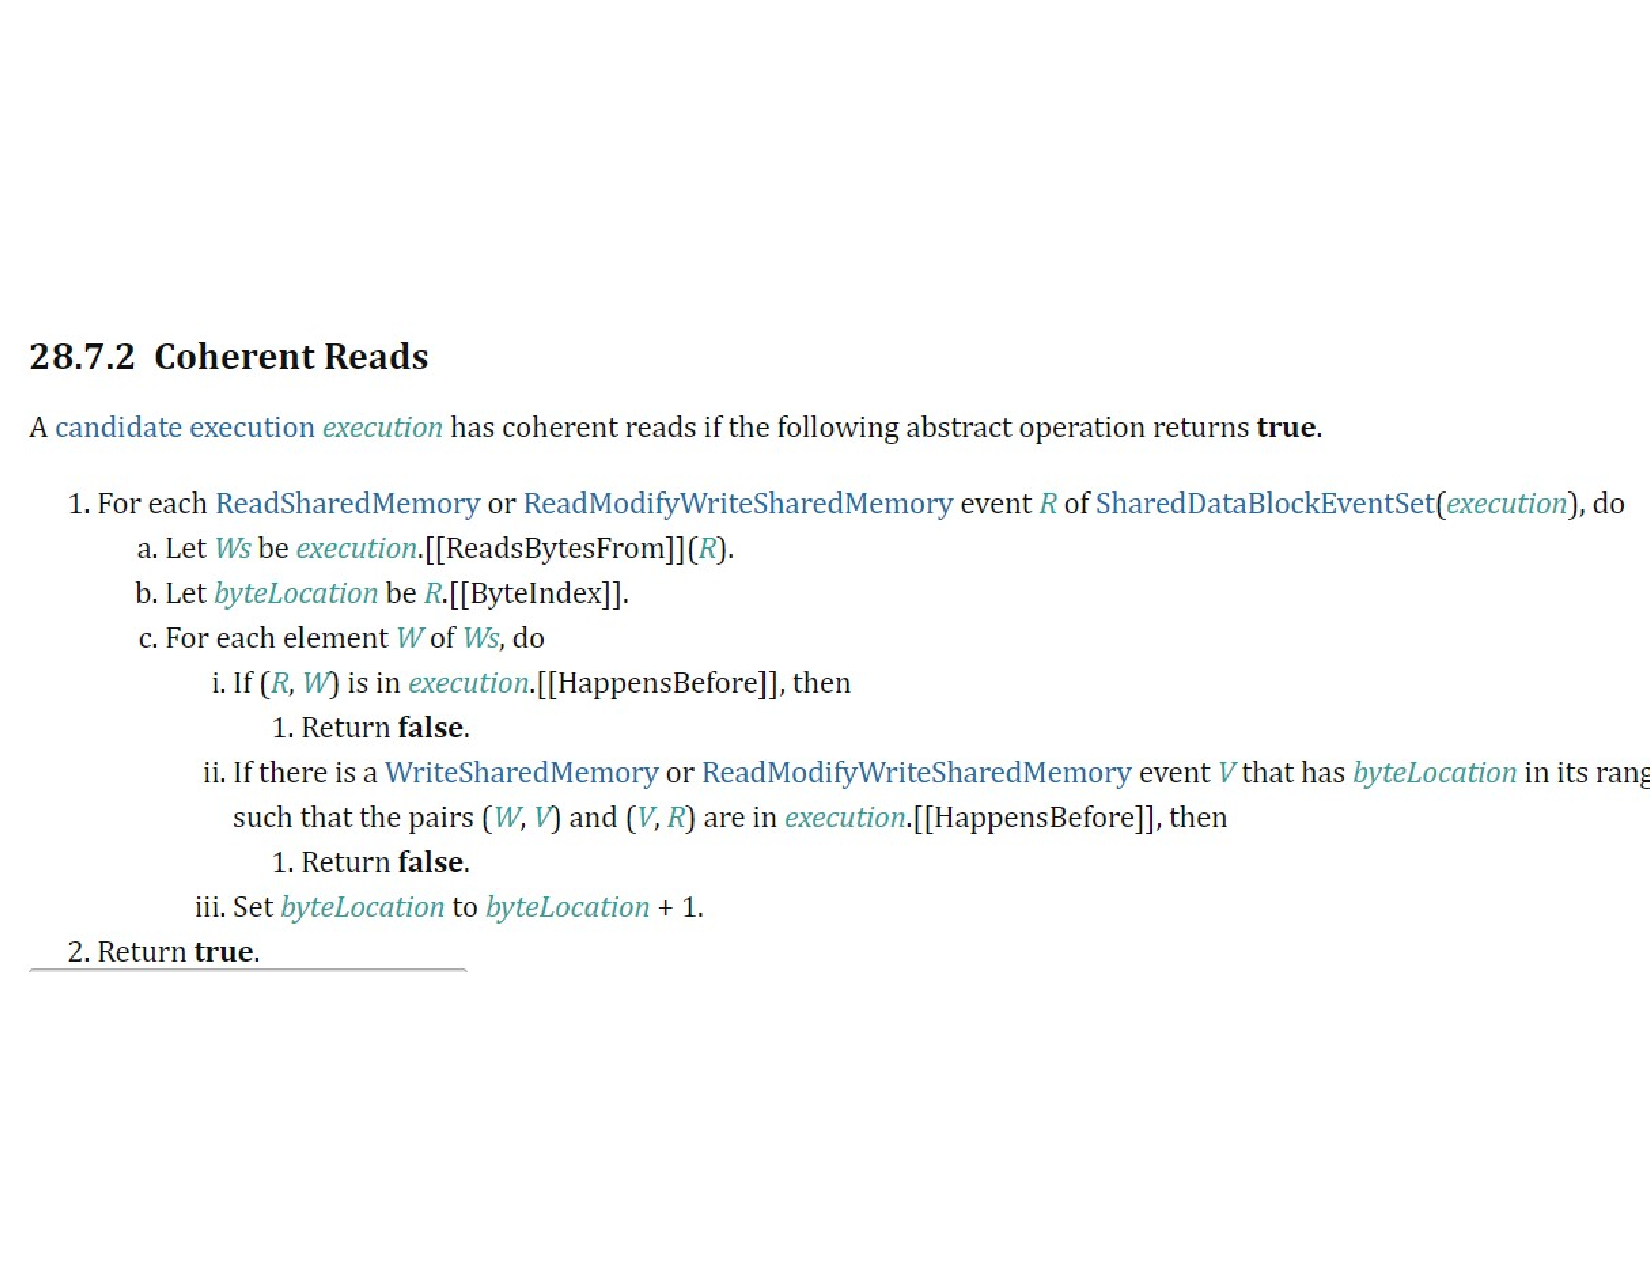
\includegraphics[scale=0.6]{3.ECMAScriptMemoryModel/ECMAScriptStdCoherentReads.pdf}
        \caption{The ECMAScript specification for Coherent Reads.}
        \label{model:Std1}
    \end{figure}
    The definition in Figure~\ref{model:Std1} is specified in terms of a return value from an abstract operation. 
    Understanding this requires one to know the definitions for \textit{Ws, execution, SharedDataBlockEventSet}, etc. although this is not required to understand what the axiom is about, which informally can be stated as below in two points:
    \begin{itemize}
        \item A read's value cannot come from a write that has happened after it. 
        \item A read's value cannot come from a write that has been overwritten by some other write.  
    \end{itemize}
    Axiomatically, we define the above two constraints using binary relations that we derive (also in some sense, take directly) from the specification in Section 2 of this chapter. 
    
\paragraph{Certain Unnecessary Definitions}
    Certain abstract operations are not required to capture the semantics of the model. 
    One such example is shown in Figure~\ref{model:Std2}
    \begin{figure}[H]
        \centering 
        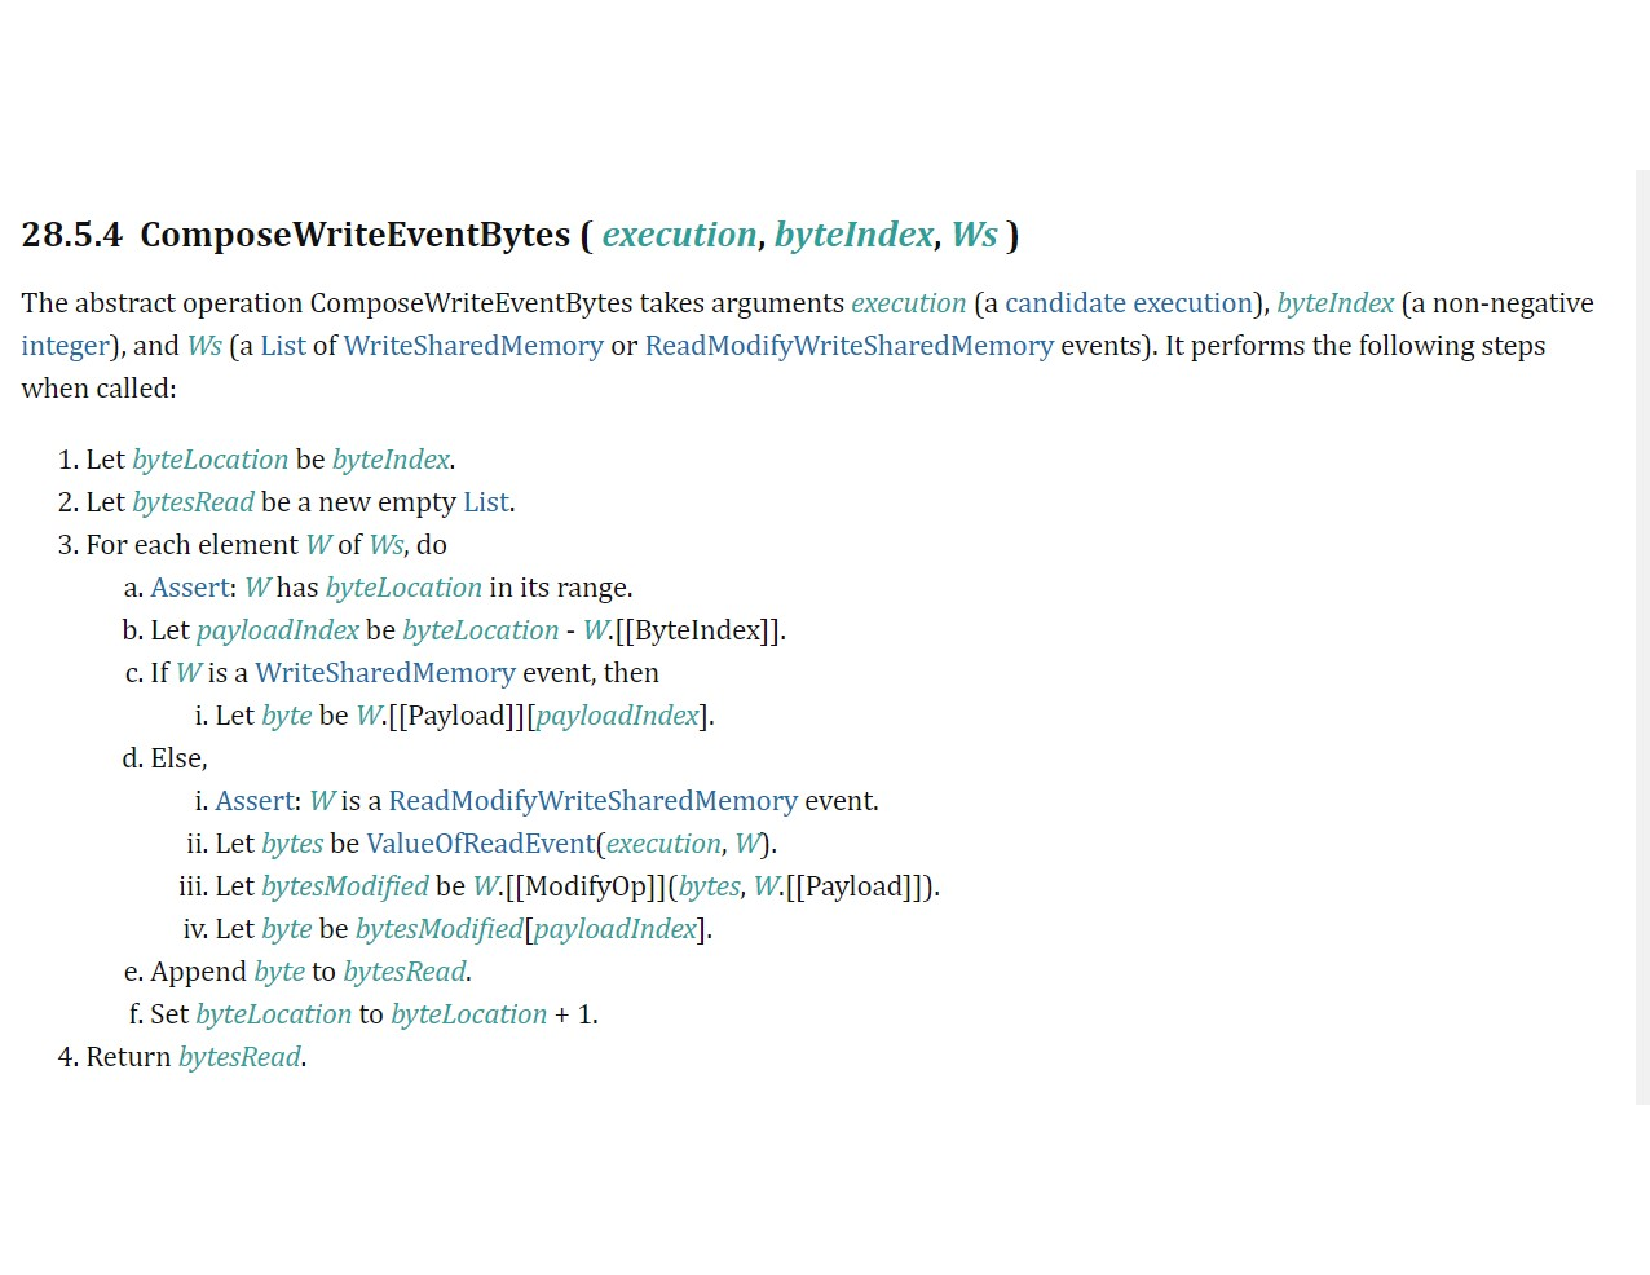
\includegraphics[scale=0.6]{3.ECMAScriptMemoryModel/ECMAScriptStd.pdf}
        \caption{The ECMAScript specification for Compose Write Event Bytes \cite{ECMA}.}
        \label{model:Std2}
    \end{figure}
    Figure~\ref{model:Std2} is the definition of an abstract operation. 
    Understanding this operation would require the meaning of the terms \textit{ModifyOp, Payload, Ws} and \textit{ByteIndex}. 
    In its essence, this operation determines the read-values read by a single event by collecting the values from their corresponding writes. 
    We noticed that one need not know this operation nor understand its function as it is not necessary in the axiomatic semantics of the model. 
    Other such abstract operations which may not be essential are \textit{ValueOfReadEvent} and \textit{ValidChosenReads}\cite{ECMA}. 

\paragraph{Still a bit verbose}
    
    The entire model, though algorithmic in its structure, is still quite verbose in its details, which makes it difficult to understand the model semantics. 
    Figure~\ref{model:Std3} is another \textit{axiom} from the standard. 
    \begin{figure}[H]
        \centering 
        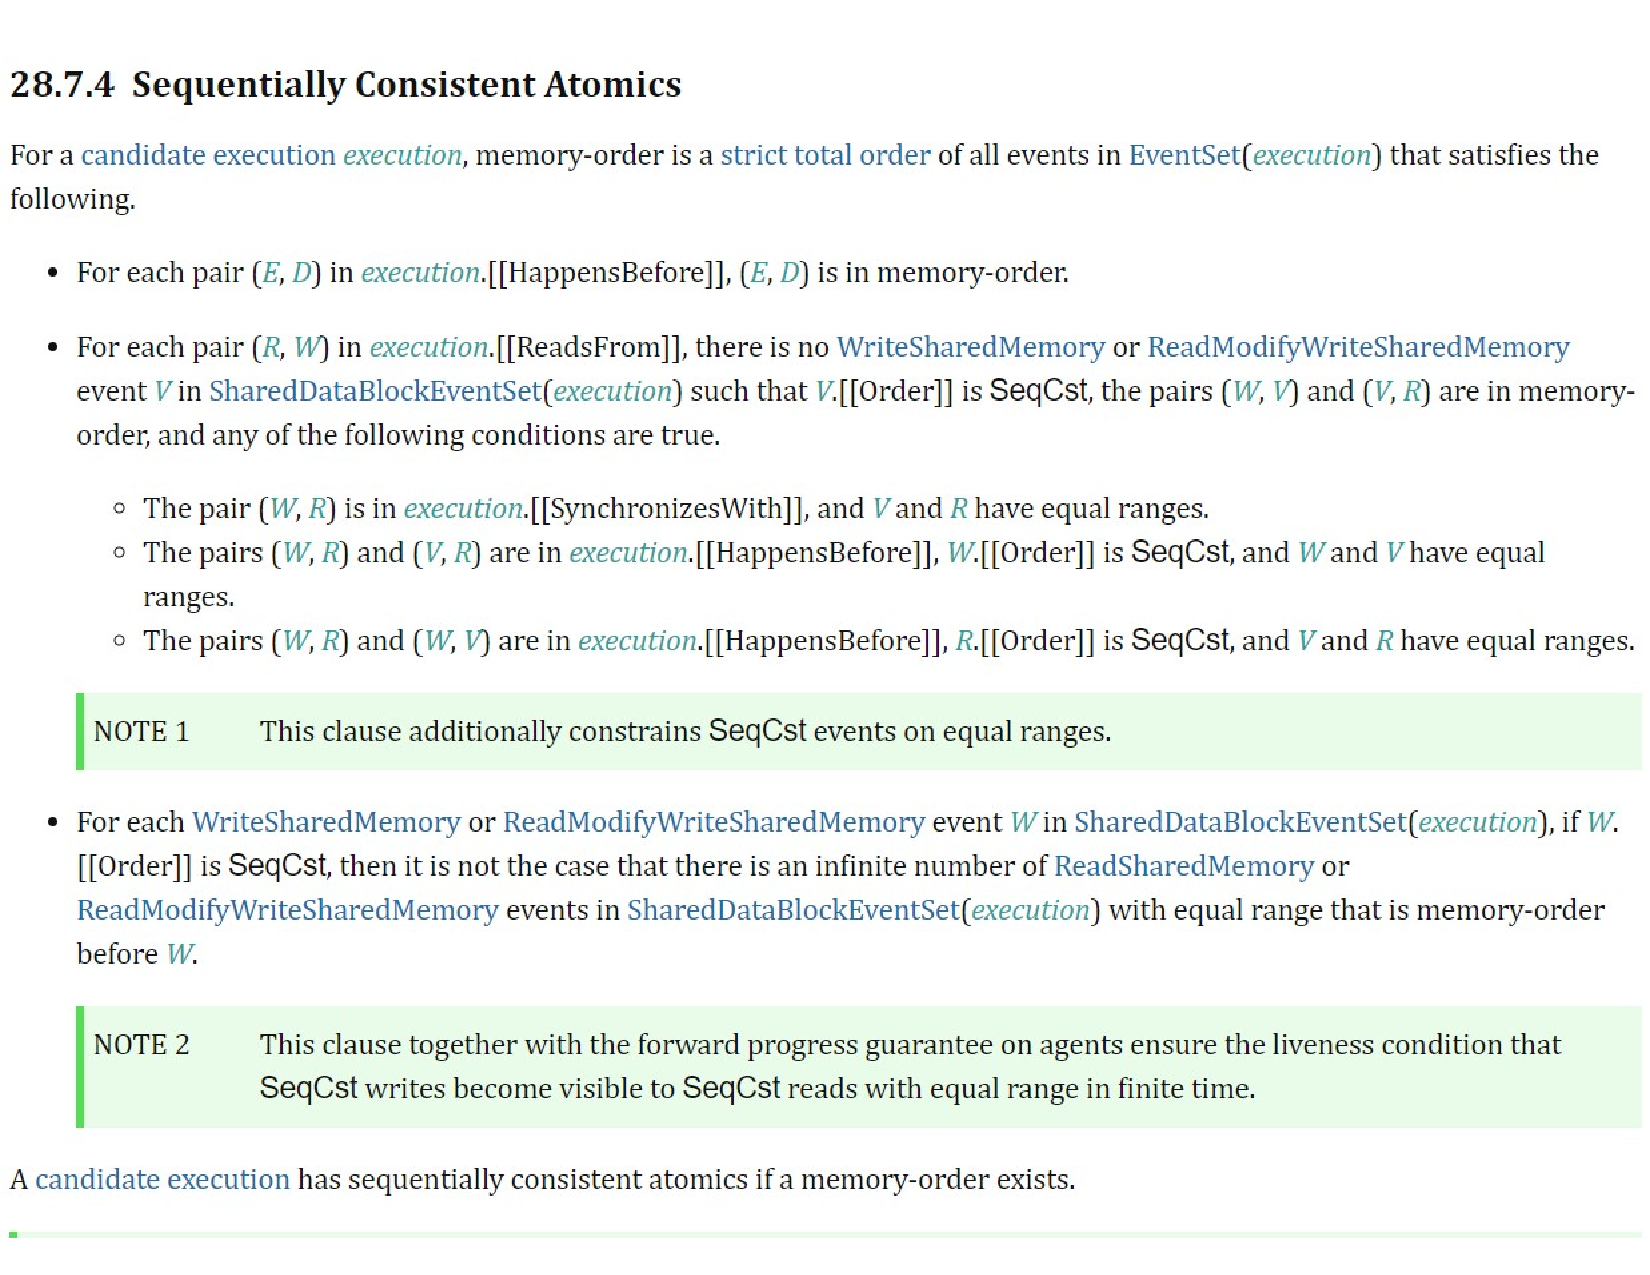
\includegraphics[scale=0.6]{3.ECMAScriptMemoryModel/ECMAScriptStdSeqCnsAt.pdf}
        \caption{The ECMAScript specification for Sequentially Consistent Atomics axiom.}
        \label{model:Std3}
    \end{figure}
    The definition in Figure~\ref{model:Std3}, is not concise enough to reason about it mathematically. 
    In addition, the part after Note1 in Figure~\ref{model:Std3} is not a semantic specification, rather a programming guideline while using 
    atomic memory accesses. 
    We will reduce the above entire axiom into three main patterns using binary relations.

Given the above concerns about the specification in the standard, we found the need to have a concise formal description of the model. 
In the following sections, we define what agents and events are, followed by several binary relations among different events.
